\section{Project Work}
\label{sec:methods}
% ======================= %
\begin{figure*}[t]
  \begin{center}
    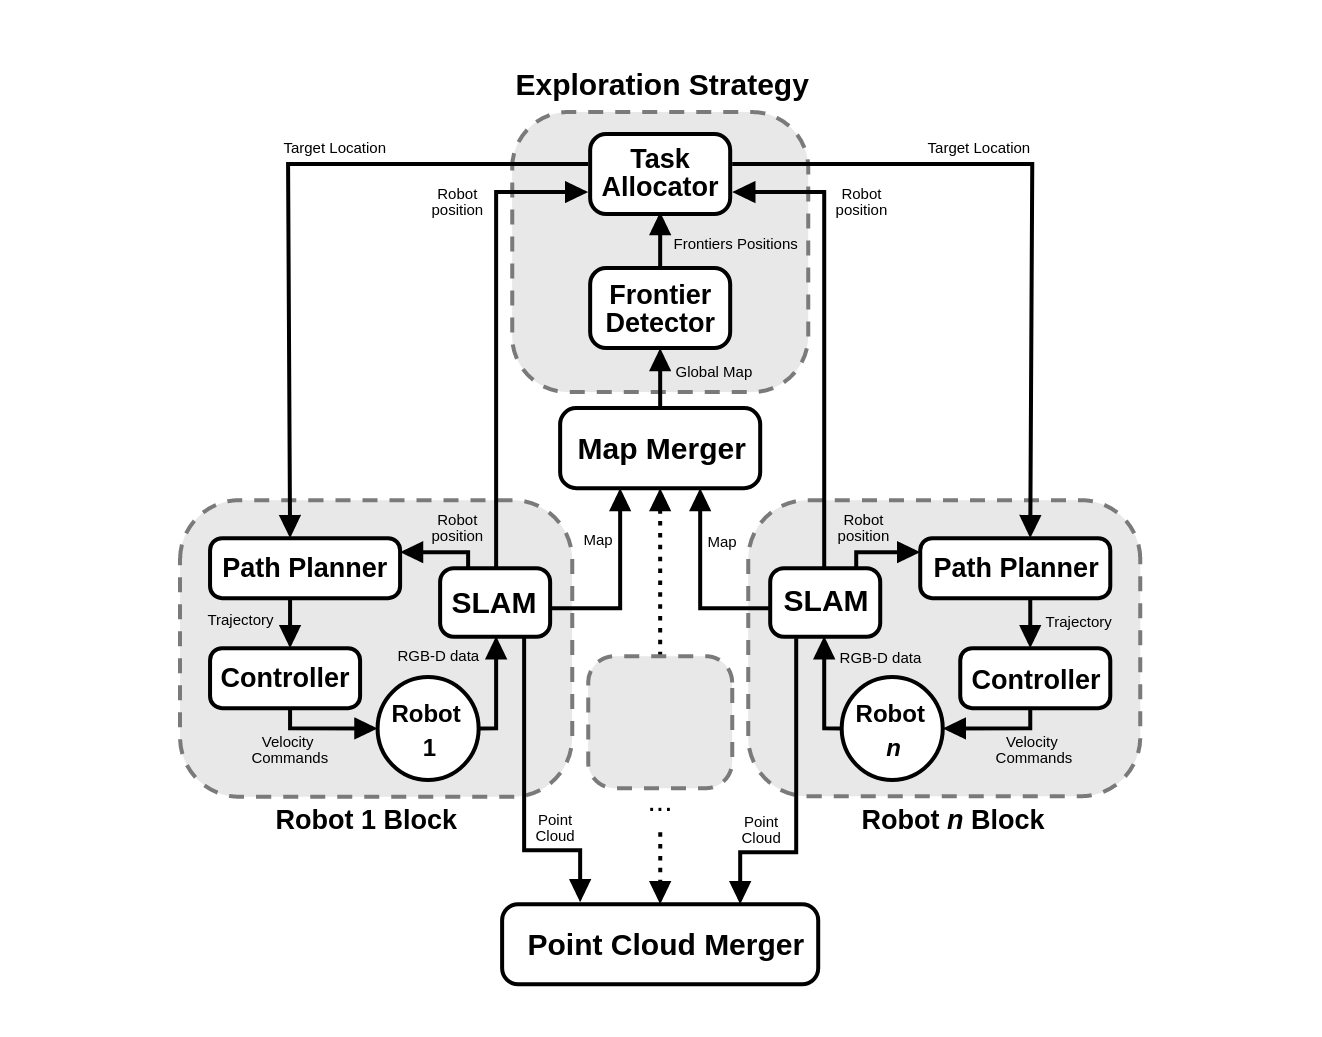
\includegraphics[width=0.7\textwidth]{img/simulation.png}
  \end{center}
  \caption[]{
    \textbf{Simulation Environment.} 
    Scheme of the multi-robot exploration. The maps built by the individual robots are merged to create a global map. Frontiers are detected and assigned to the robots as navigation goals.
  }
  \label{fig:simulation}
\end{figure*}

%
Our project work aims at developing a framework capable of achieving autonomous multi-robot exploration and mapping. Building an efficient, real time, SLAM and point-cloud manager software using an RGB-D camera is a challenging task, because solving the SLAM problem while reconstructing the point clouds requires a high computational effort. The open source Real‐Time Appearance‐Based Map (RTAB-Map) \cite{rtabmap} is the best fit for our needs given its ability to handle dense point cloud reconstruction, hybrid feature-based and graph-based SLAM, as well as the creation of an occupancy grid for navigation purposes. This solution is also focused on a loop closure detection algorithm based on the bag‐of‐words approach, where features can be any of the types included in OpenCV or ORB or more. 

This decision allowed us to create a working framework where all the map-handling functions are fully defined. Therefore, it allowed us to focus on the concepts of exploration, path planning and merging of the individual point clouds. 

\begin{comment}
To do so, we mostly cover three areas: SLAM and mapping, exploration strategy and path planning.

\end{comment}
The general scheme of the simulation model is shown in Figure \ref{fig:simulation}.

\subsection{Feature-based SLAM}

In RTAB-Map distinctive features in RGB-D data  are used to identify and track landmarks or key points in the environment, enabling the robot to create a map and estimate its own position within that map. The main steps to achieve a full map are the following:

\begin{itemize}
    \item \textbf{Feature Extraction}: visual features extraction to perform odometry and loop closure detection
    The first step in this feature-based approach is to extract distinctive features from sensor data. In the case of a camera, these features could be key points like corners or blobs. From this visual data RTAB-Map extracts distinctive visual features from each frame. These features help in identifying and matching keypoints across different frames, facilitating visual odometry and loop closure detection
    
    \item \textbf{Visual Odometry}: based on visual data and the features extracted, RTAB-Map performs visual odometry to estimate the robot's pose changes based on feature tracking between consecutive frames. This process helps the robot maintain an estimate of its position and orientation as it moves.
    
    \item \textbf{Loop Closure Detection}: Feature-based matching is a crucial step in detecting loop closures. When the robot revisits a previously visited location, the similarity of features extracted in the current frame to those in the database can indicate a loop closure event. The robot recognizes that it has been to this location before. RTAB-Map continuously compares the current sensor data with previously stored data to detect loop closures. ICP can play a role in the loop closure detection process as it helps align the current scan with previously stored scans to identify potential loop closure candidates.


    
    \item \textbf{ICP for Point Cloud Alignment}: The ICP algorithm is primarily used for aligning 3D point clouds When a potential loop closure is detected or when aligning consecutive clouds, ICP is employed to find the optimal rigid transformation (translation and rotation) that minimizes the distance between corresponding points in the two scans. This helps correct any misalignment.
    
    \item \textbf{Localization}: As the robot continues to navigate, it uses its estimated pose and the features in the map to localize itself within the environment in real-time. This enables the robot to maintain an accurate and up-to-date understanding of its position and surroundings. RTAB-Map provides real-time localization of the robot within the map. It uses the most recent sensor data and feature matching to estimate the robot's pose accurately.
    
\end{itemize}

% ======================= %
\subsection{Exploration Strategy}
In this work, we follow the idea of frontier based exploration, presented in Section \ref{sec:literature_exploration}.
Frontier-based exploration typically consists in two distinct phases: frontier detection and subsequent allocation of such frontiers to individual robots.
For the frontier detection task, we use a OpenCV-based detector. Computer vision techniques, such edge detection and contours finding, are especially effective when the input image has strong contrast between colours. This is the case of a gray-scale image describing the occupancy grid, where only three values are used for cells (free, obstacle, unexplored). The process is shown in Figure \ref{fig:cv}.
\begin{figure}[H]
\centering
\begin{tabular}{cc}
  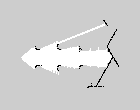
\includegraphics[width=32mm]{img/crop_input.png} &   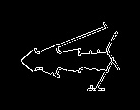
\includegraphics[width=32mm]{img/crop_edges.png} \\
(a) Starting grid & (b) Edge detection \\[6pt]
 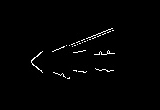
\includegraphics[width=32mm]{img/crop_res.png} &   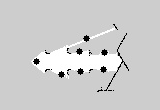
\includegraphics[width=32mm]{img/crop_points.png} \\
(c) Obstacle filtering & (d) Grid with frontiers \\
\end{tabular}
\caption{\textbf{Frontier Detection}}
\label{fig:cv}
\end{figure}
This approach allows the identification of a singular, centroid point for each frontier. In constrast, sampling-based methods would result in the identification of multiple points associated with the same frontier, necessitating additional processes like clustering for consolidation.

After the frontiers identification, the subsequent step involves the allocation of these frontiers to individual robots. In order to do so, we define a reward function $R_{ij}$ for all robot-frontiers $(i,j)$ pairs. This function serves to provide an estimate of the best frontiers for each robot to explore.
As explained in Section \ref{sec:literature_exploration}, most existing methodologies rely on the robot-frontier distance as the sole cost metric. In this work, a new reward function is introduced, which aims at finding a reasonable trade-off between costs associated with the distance and reward in the exploration. The expression is the difference between the information gain and the cost for the robot to reach that frontier:
$$ R_{ij} = I_{j} - C_{ij}$$
The length of contour describing the frontier is introduced as an indicator of the information gain. In this way, exploration of large unknown areas is also promoted, rather than the simple exploitation of nearby, smaller frontiers.
The literature suggests alternative indicators for information gain, such as the percentage of unexplored cells within a defined radius around the frontier point. However, we opt for computational efficiency by avoiding to loop over the grid multiple times. For the same reason, we do not introduce a cost linked to the length of the path to reach the assigned frontier, but rather consider only the Cartesian distance. This design enables the path planning algorithm to be invoked just once, following the frontier-robot assignment.
Heuristics can be applied to the reward calculation, in the sense that we set the reward to -inf if other robots are very close to a frontier (but not assigned to it). 

The assignment strategy follows a greedy policy, in terms of maximizing the reward. At the same time, it is ensured that no more than one robot is assigned to a specific frontier:
%%%% Greedy-Algorithm 
\begin{algorithm}
\caption{Greedy Frontier Assignment}
 \hspace*{\algorithmicindent} \textbf{Input} Robot set $P$, Frontier set $F$, Reward matrix $R$\\
 \hspace*{\algorithmicindent} \textbf{Output} $\alpha_{ij}$  assignment of robot $P_i$ to frontier $F_j$\\
\begin{algorithmic}[]
    \WHILE{$P$ is not empty}

    \IF{$F = $\,\O}
        \STATE Send robots in $P$ to initial position
    \ELSE
    
    \STATE Find $i,j$ = argmax $R_{ij}$ $\forall P_i \in P, \,\forall F_j \in F$
    \STATE $\alpha_{ij}$ = 1
    \ENDIF
    \STATE $P = P \,\backslash\, P_i$, $F = F \,\backslash\, F_j$
    \ENDWHILE{}
\end{algorithmic}
\end{algorithm}
%If the reward is defined well, then a simple greedy assignment strategy can be reasonably effective. There is no need to define a more complex policy, especially if the number of robots is not large.


\subsection{Path Planning}
In this study, we adopt the A* algorithm to address the path planning problem. Sampling-based techniques are particularly advantageous in high-dimensional spaces where the computational demands of grid-based approaches become prohibitively high. In our specific application context, we have access to a 2D grid of moderate size, making graph search methods the most suitable choice.

In the present work we present an enhanced version of the A* algorithm by integrating it with an artificial potential field generated through the Fast Marching Method (FMM) \cite{fast_marching}. 
The Fast Marching Method (FMM) \cite{fast_marching} is a numerical technique widely employed in computational physics and computer science for solving the Eikonal equation, which models the propagation of wavefronts. It returns the distance of a point from obstacles in the path. For this reason, it can be used in various domains, specifically in robotics path planning.

The original A* algorithm makes use of a priority queue to efficiently navigate through the grid. Points are extracted from the priority queue using an heuristic, which represent the total cost of the path until that point. To ensure adequate clearance from walls and obstacles, we introduce the distance computed by the FMM in the heuristic summation (Fig. \ref{fig:costmap}). This modification guides the expansion of grid-search frontiers in a direction that maintains safe distances from obstacles.

\begin{figure}[H]
  \begin{center}
    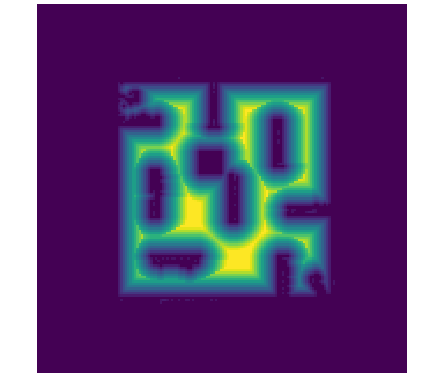
\includegraphics[width=0.4\textwidth]{img/costmap.png}
  \end{center}
  \caption[]{
    \textbf{Fast Marching Method Cost Map.} 
    Lighter squares represent safer regions, darker cells are closer to obstacles. Other robots are also considered as obstacles in the cost map.
  }
  \label{fig:costmap}
\end{figure}

Path tracking and control is achieved by the means of a simple PID pure-pursuit controller \cite{pure_pursuit}, ensuring that the robot follows the path with good flexibility.



\subsection{Point Cloud merging}
\label{sec:point_cl}
For this project work, given the capabilities of RTAB-Map but also the necessity to discover more the process behind map creation, two different approaches to Point Cloud merging where analyzed. 

\begin{algorithm}[b]
\caption{Online mapData Merging} \label{algmapData}
\begin{algorithmic}[1]
\REQUIRE Two RTAB-Map streams of \textit{mapData}, $map\_1$ and $map\_2$ 
\ENSURE Online merged point cloud: $combo\_map\_Data$
    \IF{$timerCallback$}
        \STATE \textbf{Merge maps:}
        \STATE \hspace{0.3cm} Iterate over a subset of nodes in $map\_1$ and process them in shared RTAB-Map.
        \STATE \hspace{0.3cm} Update the length of $map\_1$.

        \STATE \hspace{0.3cm} Iterate over a subset of nodes in $map\_2$ and process them in shared RTAB-Map.
        \STATE \hspace{0.3cm} Update the length of $map\_2$.

        \STATE \hspace{0.3cm} Retrieve poses and constraints from  shared RTAB-Map.
    
        \STATE \textbf{Publish merged map:}
        \STATE \hspace{0.3cm} Retrieve poses and constraints and nodes from shared RTAB-Map.
        \STATE \hspace{0.3cm} Create a new mapData type message
        \STATE \hspace{0.3cm} Publish the new message on the $combo\_map\_Data$ stream
    
    \ENDIF
\end{algorithmic}
\end{algorithm}

The first one, where the complete map is created in \textbf{real-time}, leverages directly the RTAB-Map built in functions and the suggestions given by the community \cite{rtabmapforum}. In this solution, we deploy a collaborative solution based on a hybrid \textit{decentralized} and later \textit{centralized} approach. To obtain this solution, three different instances of RTAB-Map are used: two of them are applied on the creation of two local, individual point cloud maps maps, one on each of the robots. In real time the data coming from these two point clouds is fed in a third dummy instance of RTAB-Map, where the nodes created in the two maps are merged in a sequential manner to obtain a fully merged global map. To obtain this, the requirement is to set the initial poses of the two robots such that the first visual detection is executed on the same object or scenario: this allows for an initial correct loop closure between the two maps and a optimal starting point for the creation of the whole point cloud map. The procedure follows by Algorithm \ref{algmapData}, where the most important steps are outlined. It is important to say that this code is heavily dependant on the libraries created in RTAB-Map: this leads to the creation of \textit{database} (.db) files that can only be read with a softwer connected to RTAB-Map. In order to store directly the point clouds it would be necessary to create a stream of point cloud points directly in .ply or similar file types.

\begin{algorithm}[tbh]
\caption{ICP Registration and offline PC Merging} \label{algICP}
\begin{algorithmic}[1]
\REQUIRE Two point clouds: $PC_1$ and $PC_2$, Maximum Iterations: \textit{max\_iter}
\ENSURE Aligned and merged point cloud: $final\_PC$

\STATE \textbf{tr-ICP Registration:}
    
    \FOR{ $iter$ in range($max\_iter$)}
        \STATE \textbf{Nearest Neighbor Search Using KD-Tree:}
        \STATE \hspace{0.3cm} Find nearest neighbors between $PC_1$ and $PC_2$ using a KD-tree.
        \STATE \hspace{0.3cm} Store a shuffled, partial version of the results in the $idx$ matrix.
    
        \STATE \textbf{Refine the Transformation (ICP Step):}
        \STATE \hspace{0.3cm} Refine the transformation between $PC_1$ and $PC_2$ using nearest neighbor correspondences.
        \STATE \hspace{0.3cm} Compute the transformation matrix $R_T$.
        \STATE \hspace{0.3cm} Apply $R_T$ to $PC_1$ to align it with $PC_2$.
    
    \ENDFOR

\STATE \textbf{ICP Merging Point Clouds:}
    \STATE \hspace{0.3cm} \textbf{Nearest Neighbor Search Using KD-Tree:}
        \STATE \hspace{0.6cm} Find nearest neighbors with KD-tree.
        \STATE \hspace{0.6cm} Store the total results in the $idx$ matrix.
    \STATE \hspace{0.3cm} \textbf{Merging:}
        \STATE \hspace{0.3cm} Copy one point cloud and all of its not neighbors from the other in $final\_PC$
    
\RETURN $final\_PC$
\end{algorithmic}
\end{algorithm}

Given the necessity to depend on RTAB-Map, and given the possible errors of rotation and translation between the two point clouds obtained, an additional algorithm is presented, where the manipulation is executed directly on the point clouds, without the necessity of other software. The second algorithm proposes an offline, post processing of the point clouds generated by the two instances of RTAB-Map, where a ICP algorithm is deployed for the alignment of the two maps and a duplicate point elimination in order to obtain a point cloud map without any redundant point in it. This is crucial to obtain as few points as possible in the point cloud, allowing for better storing and faster manipulation. This is depicted in  Algorithm \ref{algICP}. This algorithm leverages various libraries such as \textit{Eigen} \cite{guennebaud2010eigen} for linear algebra and matrices manipulation and \textit{nanoflann} \cite{blanco2017nanoflann} for KD-tree-based nearest neighbor search. Given these two libraries, the core of the algorithm are ICP and K-Nearest Neighbour (KNN) serach. The ICP algorithm is a common technique in computer vision and robotics for aligning two sets of 3D points. The ICP registration iteratively refines the transformation between the two point clouds, estimating both rotation and translation components. It is based on the definition of the closest points between two maps, and this is done through a KD-tree data structure. KD-trees are used for nearest neighbor search, which is a fundamental operation in point cloud processing. In this code, the KD-tree is built using the 3D spatial coordinates of one of the point clouds, allowing for fast nearest neighbor queries. The KNN functionality comes into play when searching for the nearest neighbors of points from the other point cloud. By performing KNN searches using the KD-tree, the code efficiently identifies candidate corresponding points between the two point clouds. These initial correspondences are then refined through the iterative ICP registration process, ultimately leading to an accurate alignment and merging of the point clouds. KNN is a critical component in finding these initial correspondences, which are essential for the success of the registration algorithm. The incorporation of both KNN search and ICP map reconstruction allows also to avoid overlapping points in the final point cloud, leading to more uniform density in the final merged map, as it can be seen in Figure \ref{fig:example}.

